 	\documentclass[10pt,letterpaper]{report}
\usepackage[utf8]{inputenc}
\usepackage{amsmath}
\usepackage{amsfonts}
\usepackage{amssymb}
\usepackage{graphicx}
\usepackage{subfig}
\author{Brandon Houghton}
\begin{document}
	
	Work Completed:
	
	This period we worked on training models on the pendulum and turbulence data, as well as integrating our linear model of known energies to inform a hyper-parameter sweep. 
	Preliminary results on pendulum models shows good network performance showing that the network is able to learn a non trivial invariant over simulated pendulum. These learned invariants will then be compared against functions of known pendulum energies to determine if the learned invariant is a linear function of known invariants. 
	Turbulence data has been adapted for loading into deep models. Available data did not come packaged with a time derivative term thus this term is calculated using finite differences over two points. This is assumed to be accurate enough for training, however if issues arise with learned invariants, efforts will be made to calculate the numeric derivative of charge over time more precisely.
	Orbital hyper-parameter sweeps have returned mostly negative results with the learned linear functions having zero co-efficients for terms related to known invariants. This implies that the distribution of the learned invariant over these models is not a linear combination of known invariants which contradicts previous results. This is easily explained by a bad hyper-parameter space, or an overly complex network. Additional hyper-parameter sweeps are being conducted to discover a better hyper-parameter space that recovers invariants more closely related to the hamiltonian and angular momentum of orbital bodies.
	
	
	



\begin{figure}
	\centering
	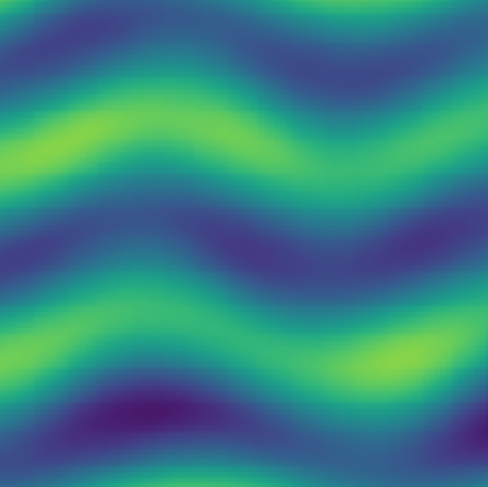
\includegraphics[width=0.3\linewidth]{./images/turb_sample_1}
	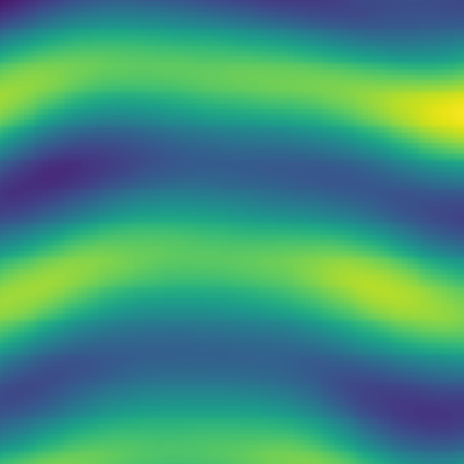
\includegraphics[width=0.3\linewidth]{./images/turb_sample_2} \\ 
	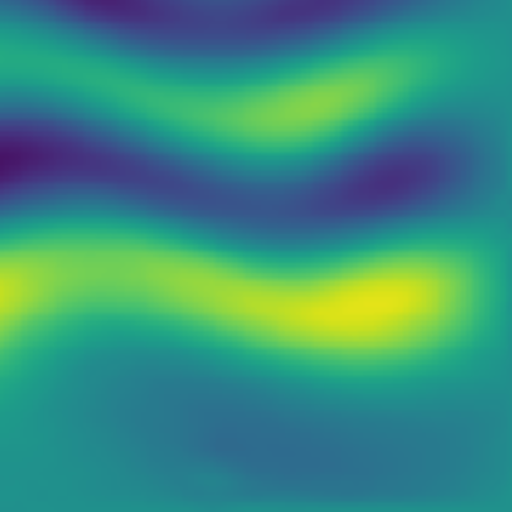
\includegraphics[width=0.3\linewidth]{./images/turb_sample_3}
	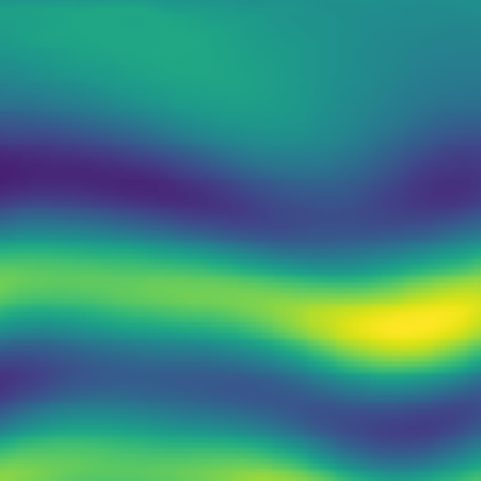
\includegraphics[width=0.3\linewidth]{./images/turb_sample_4}
	\caption{Samples at t=0 of sections of turbulence data}
	\label{fig:turbsamps}
\end{figure}






\end{document}